\documentclass[10pt,twocolumn]{article}

\usepackage[margin=0.85in]{geometry}
\usepackage{amsmath,amssymb}
\usepackage{booktabs}
\usepackage{microtype}
\usepackage[hidelinks]{hyperref}
\usepackage{titlesec}
\usepackage{enumitem}
\usepackage{listings}
\usepackage{xcolor}
\usepackage{graphicx}

\titlespacing*{\section}{0pt}{1.1ex plus .2ex}{0.6ex}
\titlespacing*{\subsection}{0pt}{0.9ex plus .2ex}{0.4ex}
\setlist{nosep,leftmargin=1.3em}

\lstset{
  basicstyle=\ttfamily\footnotesize,
  breaklines=true,
  frame=single,
  framesep=4pt,
  xleftmargin=2pt,
  columns=fullflexible,
  keepspaces=true,
  backgroundcolor=\color{gray!6},
}

\newcommand{\code}[1]{\texttt{#1}}

\title{\vspace{-3.5em}\textbf{EigenKache: Attention-Conditioned Landmark Compression\\ for Long-Context KV Caches}}
\author{Aryan Putta\\ \small Rutgers University \quad \texttt{aryansputta@gmail.com}}
\date{\small Draft v0.1 (work in progress)}

\begin{document}
\maketitle

\begin{abstract}
\noindent
Long-context transformer decoding is bottlenecked by the key/value (KV) cache,
whose size grows linearly with sequence length. Existing approaches reduce this
cost by improving allocation (PagedAttention), evicting low-importance tokens
(H2O, SnapKV, StreamingLLM), or budgeting across layers and offload paths
(LayerKV, FlowKV). Eviction permanently discards old context: under a hard
memory budget, long-range evidence that is individually low-salience but
collectively informative is lost. EigenKache reframes the cold region of the KV
cache as a \emph{streaming compression} target rather than an eviction target.
It keeps attention-sink tokens and the hot decode tail exact, and replaces the
cold middle with a small set of attention-mass-balanced \emph{landmarks}: each
landmark is a salience-weighted summary of an equal-attention-mass segment of
the cold region. The representation is deliberately \emph{structured}
(contiguous segments, fixed budget) so it maps to regular, fusible GPU memory
access rather than irregular gather. We describe the method, a CPU reference
implementation that exactly reproduces the partition-and-summarize math, and a
two-regime fidelity study against eviction baselines. On i.i.d.\ random traces,
landmark compression does not beat importance eviction---expected, since random
KV has no redundant structure. On structured traces whose cold region is
low-rank (a controlled stand-in for real long-context redundancy), landmark
compression wins at every budget, while salience eviction degrades by repeatedly
selecting near-duplicate tokens. This isolates the mechanism---compression wins
exactly when redundancy exists---and motivates the central experiment, in
progress: measuring recall fidelity and end-to-end decode latency/memory on real
Qwen and Llama long-context traces against vLLM and SGLang.
\end{abstract}

\section{Introduction}
Autoregressive decoding caches per-token keys and values so that each new token
attends to all previous ones without recomputation. The cache size is
$2 \cdot L \cdot H \cdot d \cdot n \cdot b$ bytes (layers $L$, heads $H$, head
dim $d$, sequence length $n$, dtype bytes $b$), which at long context dominates
both HBM capacity and the memory traffic of attention. Serving systems therefore
spend significant effort keeping the KV cache small.

Three families of techniques are common. \textbf{(1) Allocation / layout.}
PagedAttention removes fragmentation by paging KV blocks, improving utilization
without changing what is stored. \textbf{(2) Eviction.} H2O, SnapKV, and
StreamingLLM decide which tokens survive a budget using accumulated attention or
recency, then drop the rest. \textbf{(3) Budget routing.} LayerKV and
FlowKV/KVDirect allocate or transport KV across layers, offload tiers, and
disaggregated workers.

These are complementary and effective, but eviction-based methods share a
structural limit: \emph{once a token is dropped, the evidence it carried is
gone.} Under heavy budget pressure, the cold middle of a long context is exactly
where many individually-unremarkable tokens still collectively matter (e.g.\
retrieval-style recall across a long document). Dropping them trades recall for
memory in a way that cannot be recovered later in the decode.

\paragraph{EigenKache's stance.} Old KV state has a third option besides
\emph{exact}, \emph{evicted}, and \emph{offloaded}: keep a \emph{compact summary
aligned with future attention demand}. Concretely, EigenKache (1) preserves the
first $S$ sink tokens exactly, (2) preserves the last $T$ hot-tail tokens
exactly, (3) scores the cold middle by recent-query attention salience, (4)
partitions the middle into equal-attention-mass segments, and (5) replaces each
segment with one salience-weighted landmark key/value pair, optionally keeping
the few highest-salience middle tokens exact. The result fits a fixed budget
while retaining global anchors, near-term decode locality, and a compressed
summary of older evidence.

\paragraph{Contributions.}
\begin{itemize}
\item A KV-cache method that treats the cold region as a structured compression
target (attention-mass landmarks) rather than a set of survivors.
\item A CPU reference implementation and an apples-to-apples benchmark harness
that measures compression ratio, KV bytes saved, attention-output L2 / cosine
fidelity, and runtime across \code{full}, \code{window}, \code{h2o\_like}, and
\code{landmark} policies at matched budgets.
\item A proof-of-concept fidelity study and an honest negative finding on
synthetic random traces, which scopes the conditions under which compression
should beat eviction and defines the real-model evaluation that follows.
\end{itemize}

\section{Background and Related Work}
\textbf{Attention and HBM traffic.} FlashAttention shows that attention is
memory-movement-bound; a useful KV optimization must reduce real HBM traffic,
not only token count on paper. EigenKache's landmark layout is contiguous so the
compress-and-attend path can be tiled and fused.

\textbf{Paging.} PagedAttention fixes allocation waste but not the
\emph{semantic} cost of a hard budget; it stores the same tokens, just better.

\textbf{Eviction.} H2O keeps ``heavy hitter'' tokens by accumulated attention;
SnapKV selects tokens via recent-query attention pooling; StreamingLLM keeps
sink tokens plus a recent window. All discard the rest. EigenKache reuses the
sink + tail structure of StreamingLLM and the recent-query salience signal of
SnapKV/H2O, but \emph{summarizes} the middle instead of dropping it.

\textbf{Budget routing and transport.} LayerKV budgets across layers and
offload; FlowKV/KVDirect reduce disaggregated transfer cost. A smaller
semantically-useful representation should compound with these, since there is
less state to move.

The gap EigenKache targets: \emph{existing systems improve layout, routing,
offload, or eviction, but still lose long-range evidence when old context must
fit a hard budget.}

\section{Method}
Let a single head's cached state be $K, V \in \mathbb{R}^{n \times d}$ for $n$
cached tokens of head dimension $d$, with recent query vectors
$Q \in \mathbb{R}^{q \times d}$ used to estimate salience.

\paragraph{Salience.} Define per-token salience as the mean recent-query
attention mass:
\begin{align}
A &= \mathrm{softmax}\!\left(\tfrac{Q K^\top}{\sqrt{d}}\right) \in \mathbb{R}^{q \times n}, &
s_j &= \tfrac{1}{q}\textstyle\sum_{i} A_{ij}.
\end{align}

\paragraph{Region split.} Given a token budget $B$, reserve the $S$ sink tokens
$[0,S)$ and the $T$ tail tokens $[n{-}T, n)$ as exact. The cold middle is
$M = [S, n{-}T)$ with middle budget $B_m = \max(0, B - S - T)$.

\paragraph{Exact carve-out.} A small fraction of $B_m$ keeps the
highest-salience cold tokens exact (reference: $\lfloor B_m/4 \rfloor$, clamped
to $[1, |M|{-}1]$). The remaining budget $B_m - e$ funds $L$ landmarks.

\paragraph{Equal-attention-mass landmarks.} Let the remaining cold tokens (in
original order) have salience $w_1\ldots w_m$ with cumulative mass
$C_k = \sum_{j \le k} w_j$ and total $C_m$. To produce $L$ landmarks, place
$L{+}1$ evenly spaced mass boundaries $b_i = i\,C_m/L$, and assign cold token $k$
to landmark $i$ iff $C_{k-1} < b_i \le C_k$ (via \code{searchsorted}). Each
landmark is the salience-weighted mean of its segment:
\begin{equation}
\hat{K}_i = \!\!\sum_{k \in \mathrm{seg}_i}\!\! \frac{w_k}{\sum w}\, K_k,
\qquad
\hat{V}_i = \!\!\sum_{k \in \mathrm{seg}_i}\!\! \frac{w_k}{\sum w}\, V_k.
\end{equation}
This is the key design choice: segments carry \emph{equal attention mass}, not
equal token count, so high-salience regions get finer landmarks and flat regions
get coarse ones. The compressed cache is the concatenation
$[K_{\text{sink}}; K_{\text{exact}}; \hat{K}; K_{\text{tail}}]$ (and likewise for
$V$), giving a fixed size of $S + e + L + T$ entries regardless of $n$.

\paragraph{Why structured.} Landmarks are contiguous spans over the cold region,
so the gather-compress-attend path stays regular. Unstructured per-token
sparsity tends to hurt real GPU throughput because access becomes irregular;
EigenKache trades a little theoretical flexibility for memory-access regularity
that a fused kernel can exploit.

\section{Implementation}
The repository contains a \textbf{CPU reference}
(\code{src/eigenkache/policies.py}) implementing \code{full}, \code{window}
(StreamingLLM-style sink+window), \code{h2o\_like} (salience eviction), and
\code{landmark} (this method) behind a common \code{run\_policy} interface, with
a benchmark harness (\code{bench.py}) that records compression ratio, KV bytes
saved, attention-output L2 / cosine fidelity, and runtime. A \textbf{CUDA-first
design} (\code{cuda/attention\_landmark\_kernel.cu}) targets fused landmark
attention with shared-memory tiling, so compression and decode are scheduled as
one dataflow rather than separate passes. The CPU reference is the source of
truth for correctness; the CUDA path is for the latency/throughput claims in the
planned evaluation.

\section{Experimental Setup}
\paragraph{Proof-of-concept (done).} A synthetic KV trace ($n{=}96$, $d{=}128$,
$q{=}12$) is compressed to matched budgets by every policy, and we measure the
fidelity of the resulting attention output against the exact (\code{full})
output. This validates that the harness measures the right thing and that
landmark compression is numerically well-behaved.

\paragraph{Real-model evaluation (in progress).} The central experiment fixes the
gaps above: \textbf{Models:} Qwen2.5-7B and Llama-3.1-8B (real attention traces,
GQA). \textbf{Datasets:} LongBench and RULER for recall-sensitive long-context
tasks; PG19 for perplexity under budget. \textbf{Baselines:} vLLM and SGLang with
(a) full cache, (b) StreamingLLM window, (c) H2O/SnapKV eviction---all at matched
KV budgets. \textbf{Metrics:} task accuracy / perplexity vs KV budget; decode
latency and peak KV memory; HBM traffic from the fused kernel. The hypothesis is
explicit: on real traces whose cold region is structurally redundant,
attention-mass landmarks preserve recall at a given budget better than eviction,
at competitive latency.

\section{Results}
We report attention-output cosine similarity to the exact cache at three matched
budgets (higher is better). At a given budget all policies hit identical
compression ratios and KV-byte savings (e.g.\ $4.0\times$ / 75\% bytes saved at
25\% retention), so the comparison is purely about \emph{fidelity per byte}. We
run two regimes that differ only in the statistical structure of the cold
region (Figure~\ref{fig:regimes}).

\begin{figure*}[t]\centering
  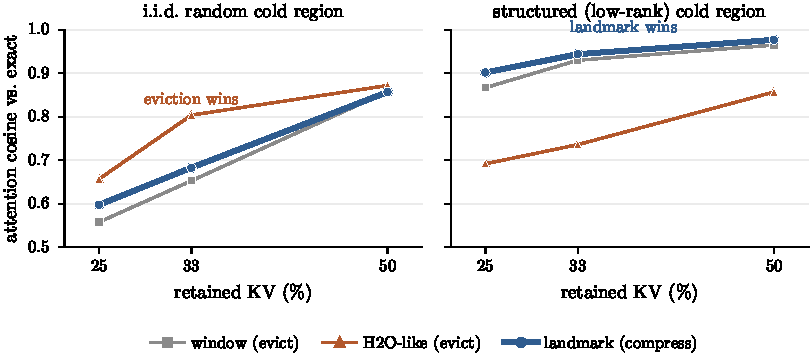
\includegraphics[width=0.92\textwidth]{figs/regimes.pdf}
  \caption{Landmark compression beats eviction only when the cold region is
  redundant. Attention-output cosine vs.\ the exact cache, at matched KV budgets.
  Left, an i.i.d.\ random cold region: H2O-like eviction leads (0.657 vs landmark
  0.598 at 25\% retained). Right, a structured low-rank cold region: landmark
  leads at every budget (0.902 vs 0.692 at 25\%), and H2O degrades by selecting
  near-duplicate tokens. Same method uses the same color and marker in both
  panels.}
  \label{fig:regimes}
\end{figure*}

\paragraph{Regime 1: i.i.d.\ random trace ($n{=}96$, $d{=}128$).} Each token is
independent Gaussian noise (Table~\ref{tab:random}). Here importance eviction
(\code{h2o\_like}) wins: with no redundancy, averaging tokens into a landmark
destroys as much as it preserves, while eviction keeps some vectors exact.

\begin{table}[t]
\centering\small
\begin{tabular}{lccc}
\toprule
Retained (comp.) & window & h2o\_like & landmark \\
\midrule
25\% ($4.0\times$) & 0.558 & \textbf{0.657} & 0.598 \\
33\% ($3.0\times$) & 0.653 & \textbf{0.804} & 0.683 \\
50\% ($2.0\times$) & 0.858 & \textbf{0.872} & 0.857 \\
\bottomrule
\end{tabular}
\caption{Cosine similarity vs.\ exact --- i.i.d.\ random trace. No redundant
structure: eviction wins.}
\label{tab:random}
\end{table}

\paragraph{Regime 2: structured trace ($n{=}512$, $d{=}128$).} The cold middle is
drawn from a small set of topic centroids plus small noise---a controlled
stand-in for the low-rank, redundant structure real long-context KV exhibits
(repeated topics, low intrinsic rank). Sink and tail tokens remain distinct.
Here landmark compression \emph{wins at every budget}
(Table~\ref{tab:structured}), and by a widening margin as the budget tightens.
Notably \code{h2o\_like} now does \emph{worse} than a plain window: salience
eviction repeatedly picks near-duplicate high-salience tokens from the same
cluster and loses topic coverage, whereas attention-mass landmarks place one
summary per topic and preserve coverage.

\begin{table}[t]
\centering\small
\begin{tabular}{lccc}
\toprule
Retained (comp.) & window & h2o\_like & landmark \\
\midrule
25\% ($4.0\times$) & 0.867 & 0.692 & \textbf{0.902} \\
33\% ($3.0\times$) & 0.930 & 0.736 & \textbf{0.944} \\
50\% ($2.0\times$) & 0.965 & 0.857 & \textbf{0.977} \\
\bottomrule
\end{tabular}
\caption{Cosine similarity vs.\ exact --- structured (low-rank) cold region.
Compression wins where redundancy exists.}
\label{tab:structured}
\end{table}

\paragraph{Takeaway.} The two regimes isolate the mechanism precisely:
\emph{landmark compression beats eviction exactly when the cold region is
redundant, and only then.} Random noise (Regime 1) favors eviction; structured
redundancy (Regime 2) favors compression. Real long-context traces are far
closer to Regime 2 than Regime 1, which is why the real-model evaluation
(Section~5) is expected to favor EigenKache---but that claim is only settled by
measuring it on real traces, not by either synthetic regime alone. The
structured-trace experiment is reproducible via
\code{scripts/structured\_trace\_experiment.py}.

\section{Limitations and Next Steps}
The decisive accuracy/latency claims require the real-model benchmark; current
numbers are a CPU-reference proof of concept on synthetic data and should not be
read as end-to-end wins. The CUDA fused kernel is in design; latency and
HBM-traffic numbers depend on it landing and being profiled against vLLM/SGLang.
Salience uses a recent-query window; sensitivity to window size and to GQA head
grouping is unmeasured. The exact-carve-out fraction ($B_m/4$) is a heuristic and
should be swept.

\textbf{Immediate next steps:} (1) capture real per-layer KV traces from
Qwen/Llama on LongBench; (2) run the matched-budget fidelity study on those
traces; (3) wire the landmark policy behind the torch hook for end-to-end
decode; (4) profile the CUDA landmark-attention kernel for HBM traffic.

\section*{References}
\small
\begin{enumerate}[label={[\arabic*]}]
\item Vaswani et al. \emph{Attention Is All You Need}. NeurIPS 2017.
\item Dao et al. \emph{FlashAttention}. NeurIPS 2022.
\item Kwon et al. \emph{Efficient Memory Management for LLM Serving with PagedAttention (vLLM)}. SOSP 2023.
\item Zhang et al. \emph{H2O: Heavy-Hitter Oracle for Efficient Generative Inference}. NeurIPS 2023.
\item Li et al. \emph{SnapKV: LLM Knows What You Are Looking For Before Generation}. 2024.
\item Xiao et al. \emph{Efficient Streaming Language Models with Attention Sinks (StreamingLLM)}. ICLR 2024.
\item \emph{LayerKV}, \emph{FlowKV}, \emph{KVDirect}: KV budgeting and transport.
\item Bai et al. \emph{LongBench}; Hsieh et al. \emph{RULER}; Rae et al. \emph{PG19}.
\end{enumerate}

\end{document}
